

\subsection{Ladder-Lottery Realization}

In their paper \textbf{Ladder-Lottery Realization} the authors provide 
a rather interesting puzzle in regards to ladder lotteries. The puzzle 
is known as the ladder-lottery realization problem. In order to understand
the problem, one must know what a \emph{multi-set} is. A \emph{multi-set}
is a set in which an element appears more than once. The exponent 
above the element indicates the number of times it appears in the set.
For example, given the following multi-set, $\{3^{2}, 2^{4}, 5^{1}\}$ 
the element $3$ appears twice in the set, the element $2$ appears four times
in the set and the element $5$ appears once in the set.
The ladder-lottery realization puzzle asks, given an arbitrary starting permutation 
and a multi-set of bars, 
is there a \emph{non-optimal} ladder lottery for the arbitrary permutation
that uses every bar in the multi-set the number 
of times it appears in the  multi-set. 
For an example of an affirmative solution to the ladder lottery realization problem, see figure --fig ref --.


\begin{figure}[!htp]
    \begin{center}
        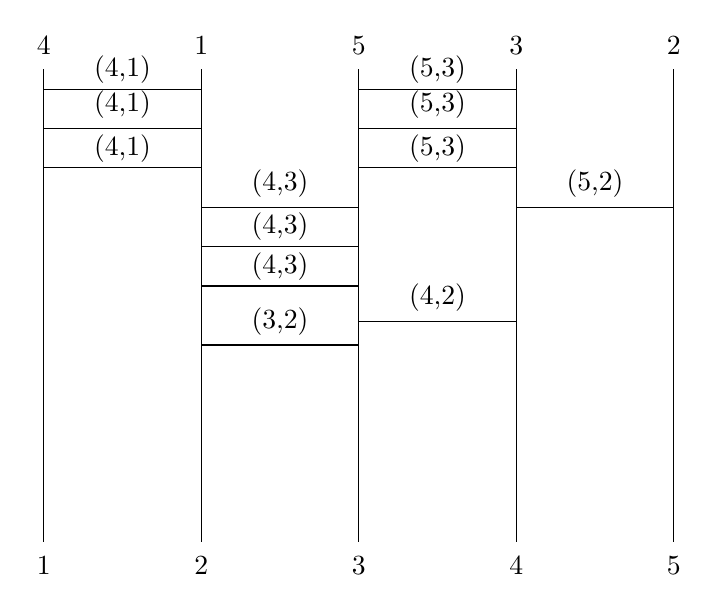
\begin{tikzpicture}
            \draw (0, 0) to (0, 6);
                \node at(0, -0.3){1};
                \node at(0, 6.3){4};
            \draw(2, 0) to (2, 6);
                \node at(2, -0.3){2};
                \node at(2, 6.3){1};
            \draw(4, 0) to (4, 6);
                \node at(4, 6.3){5};
                \node at(4, -0.3){3};
            \draw(6, 0) to (6, 6);
                \node at(6, 6.3){3};
                \node at(6, -0.3){4};
            \draw(8, 0) to (8, 6);
                \node at(8, 6.3){2};
                \node at(8, -0.3){5};

            %%draw the bars
                \node at(1, 6){(4,1)};
                    \draw(0, 5.75) to (2, 5.75);
            \draw(0, 5.25) to (2, 5.25);
                \node at(1, 5.55){(4,1)};
            \draw(0, 4.75) to (2, 4.75);
                \node at(1, 5){(4,1)};

            \draw(4, 5.75) to (6, 5.75);
                \node at(5, 6){(5,3)};
            \draw(4, 5.25) to (6, 5.25);
                \node at(5, 5.55){(5,3)};
            \draw(4, 4.75) to (6, 4.75);
                \node at(5, 5){(5,3)};

            \draw(2, 4.25) to (4, 4.25);
                \node at (3, 4.55){(4,3)};
            \draw(2, 3.75) to (4, 3.75);
                \node at (3, 4){(4,3)};
            \draw(2, 3.25) to (4, 3.25);
                \node at (3, 3.5){(4,3)};
            
            \draw(2, 2.5) to (4, 2.5);
                \node at(3, 2.8){(3,2)};
            
            \draw(4, 2.8) to (6, 2.8);
                \node at (5, 3.1){(4,2)};
            \draw(6, 4.25) to (8, 4.25);
                \node at (7, 4.55){(5,2)};
            
        \end{tikzpicture}
    \end{center}
      


    \caption{An affirmative solution to the Ladder Lottery Realization Problem
    given a starting perumtation $(4,1,5,3,2)$ and the multi set 
    $\{(4,1)^{3}, (4,3)^{3}, (4,2)^{1}, (5,4)^{2}, (5,3)^{3}, (5,2)^{1},(3,2)^{1}\}$}
\end{figure}